\documentclass{article}

\usepackage[utf8]{inputenc}
\usepackage[T1]{fontenc}
\usepackage{polski}
\usepackage{indentfirst}
\usepackage{lastpage}
\usepackage{natbib}
\usepackage{graphicx} 
\usepackage{sidecap}
\usepackage{wrapfig}
\usepackage{subfig}
\usepackage{caption}



\usepackage{fancyhdr}
\pagestyle{fancy}
\fancyhf{}
\rhead{Franciszek Wysocki}
\rfoot{Strona \thepage \hspace{1pt} z \pageref{LastPage}}
\lhead{Spis treści}
\title{Specyfikacja implementacyjna projektu pt. ,,Centrum Zarządzania Szczepionkami''}
\author{}
\date{}

\begin{document}
\maketitle

\begin{flushright}
\par
\vfill
\par
{\fontsize{11}{11}\selectfont
    Wykonał: Franciszek Wysocki

    Sprawdzający: mgr inż. Paweł Zawadzki

    Data: 16-11-2020
}
\end{flushright}
\thispagestyle{empty}

\newpage

\tableofcontents

\newpage

\section{Cel dokumentu}
{\fontsize{13}{13}\selectfont
    Celem niniejszego dokumentu jest przedstawienie szczegółów implementacyjnych do projektu pt. „Centrum Zarządzania Szczepionkami”. Zostaną opisane techniczne aspekty takie jak: środowisko deweloperskie, zasady wersjonowania, struktura projektu, wykorzystane struktury danych i algorytmy, sposoby testowania i kompilowania. 
}

\lhead{Cel dokumentu}

\section{Cel projektu}
{\fontsize{13}{13}\selectfont
    Celem projektu jest zapewnienie optymalnego sposobu dostaw szczepionek poprzez opracowanie odpowiedniego programu. Ten, dokonując analizy konkretnych danych, dostarczonych przez grupę menadżerską, powinien doprowadzić do ustalenia w jaki sposób należy przeprowadzić dostawy, aby możliwie wypełnić dzienne zapotrzebowanie wszystkich zarządzanych aptek, robiąc to jednocześnie przy najmniejszym możliwym koszcie całkowitym. Uzyskane wnioski, informujące o tym, która apteka powinna zamówić jaką ilość szczepionek od którego producenta, powinny zostać zapisane do pliku wyjściowego. Więcej szczegółów o plikach zostało zawartych w dokumencie specyfikacja funkcjonalna.

}

\section{Środowisko deweloperskie}
{\fontsize{13}{13}\selectfont
    
    \begin{itemize}
        \item Język programowania: Java 13 (JDK 13.0.2),
        \item Zintegrowane środowisko deweloperskie: IntelliJ IDEA 2020.2 (Ultimate Edition z licencją edukacyjną),
        \item Pozostałe narzędzia: Apache Maven v3.6.3, Projektor v2.4.1, git v2.17.1,
        \item o	System operacyjny: Windows 10 Home w wersji 2004 (64 bitowy),
        \item Podzespoły: Procesor: Intel(R) Core(TM) i7-8565U CPU 1.8 GHz 1.99 GHz, zainstalowana pamięć RAM: 16GB,

   
     \end{itemize}
    
 
}

    
\newpage

\section{Zasady wersjonowania}
{\fontsize{13}{13}\selectfont
    
    Wersjonowanie odbędzie się za pomocą gita (w formie dodanych tagów):

    \begin{itemize}
        \item ,,STABLE\_n'' - wersje stabilne, gdzie n = 1.0, 2.0, ...,
        \item,,FINAL\_RELEASE'' - wesja finalna,
    \end{itemize} 
    Wiadomości z ,,commitów'' będą pisane w języku angielskim i będą (krótko) opisywały co zostało dodane/zmienione od czasu poprzedniego commita. 
    
    Praca na gicie zostanie rozłożona na wiele gałęzi, aby pracować jednocześnie na wielu modułach. Łączenie gałęzi będzie wykonywane za pomocą komendy git merge.
}
\lhead{Zasady wersjonowania}



\section{Testowanie}
{\fontsize{13}{13}\selectfont
    Program będzie testowany za pomocą testów jednostkowych. Do ich pisania zostaną wykorzystane biblioteki JUnit5, AssertJ oraz Mockito. Testy będą sprawdzały poprawność działania konkretnych metod publicznych ze szczególnym naciskiem na warunki brzegowe, odporność na niepożądane warunki (takie jak np. podanie niezainicjowanej zmiennej jako argument funkcji).
    Kolejność ich uruchomienia będzie dowolna, gdyż te będą od siebie niezależne. Testy będą również powtarzalne, a ich wyniki jednoznaczne.
    Nazwy testów będą pisane zgodnie z konwencją:
    
    \texttt{ should\_expectedBehavior\_when\_stateUnderTest }
    \setlength{\parindent}{0pt}
        
    a same testy z konwencją given/when/then.
    Wszystkie testy będą znajdować się w katalogu test.
    Testy będą automatycznie uruchamiane za pomocą Mavena przed stworzeniem pliku JAR.
    Ponadto ostateczna wersja programu zostanie przetestowana manualnie dla różnych (poprawnych, jak i nie) plików wejściowych.
    \setlength{\parindent}{12pt}
}


\section{Struktura projektu}
{\fontsize{13}{13}\selectfont
    Struktura projektu będzie zgodna ze domyślną strukturą Mavena (domyślnie kod będzie znajdował się w katalogu: src/main/java (Rysunek 1), a testy: src/test/java).
    
    \begin{figure} [hbt!]
        \centering
        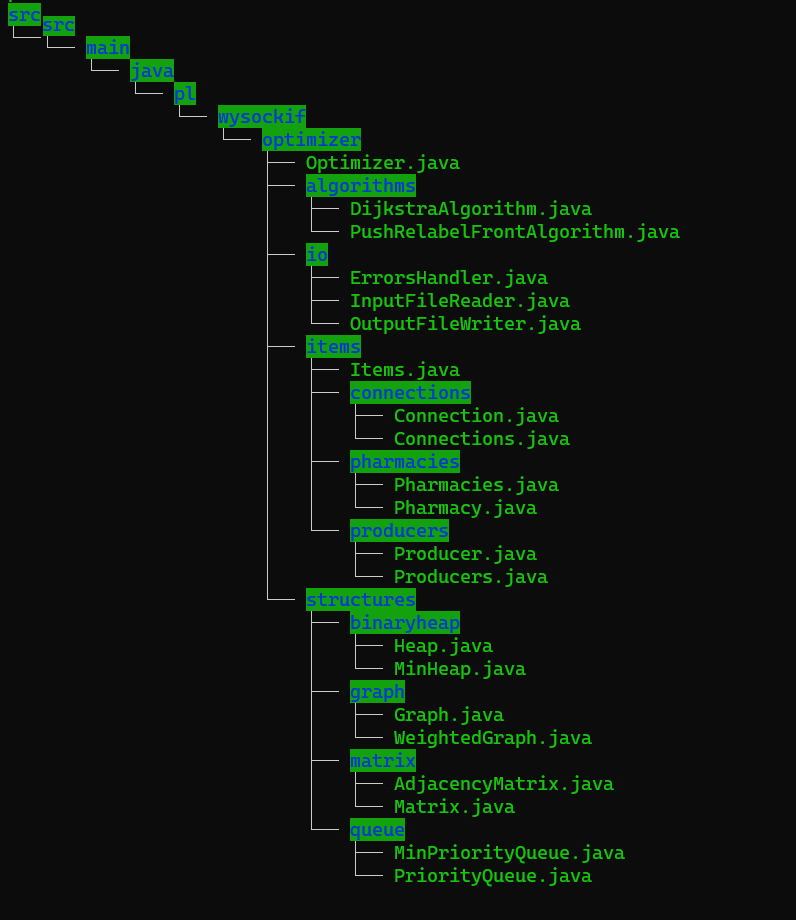
\includegraphics[width=12cm]{projectStructure.png}
      \captionof{figure}{}
    \end{figure}
    
    \newpage
    \lhead{Struktura projektu}
    Struktura klas testowych będzie analogiczna do powyższej.
}

\newpage

\section{Klasy i interfejsy}
    \subsection{Opis}
    {\fontsize{13}{13}\selectfont
        \begin{itemize}
            \item Klasa Optimizer będzie klasą główną programu i będzie ona zarządzać jego działaniem. W niej będzie znajdować się metoda main.
            \item Klasa PushRelabelFrontAlgorithm będzie zawierać metody reprezentujące algorytm ,,przemianuj i przesuń na początek’’.
            \item Klasa DijkstraAlgorithm będzie zawierać metody reprezentujące algorytm Dijkstry.
            \item Klasa InputFileReader będzie służyła do odczytu danych z pliku wejściowego.
            \item Klasa OutputFileWriter będzie służyła do zapisu danych do pliku wyjściowego.
            \item Klasa ErrorsHandler będzie posiadała zdefiniowane kody błędów i metodę wyświetlającą komunikat błędu na strumień err oraz zakończającą działanie programu z odpowiednim kodem błędu.
            \item 	Interfejs  Items będzie reprezentował pojedyncze pozycje, jakie można odczytać z pliku. Interfejs ten zostanie stworzony w celu opracowania uniwersalnej metody do odczytu atrybutów klas implementujących go - klasy: Producers, Pharmacies, Connections. Te kolejno będą posiadały listy klas Producer, Pharmacy i Connection oraz metody zapewniające operacje na całych kolekcjach.
            \item Klasa MinHeap (implementująca interfejs Heap) będzie reprezentowała kopiec z wartością najmniejszą na szczycie. Jej metody będą pozwalały na dodawanie nowych elementów i zdejmowanie istniejących. Klasa ta zostanie wykorzystana do zaimplementowania kolejki priorytetowej (klasa MinPriorityQueue z interfejsem PriorityQueue).
            \item Klasa AdjacencyMatrix (implementująca interfejs Matrix) będzie reprezentowała macierz i posłuży do przechowywania grafu (klasa WeightedGraph z interfejsem Graph).
    
        \end{itemize}
            \lhead{Klasy i interfejsy}
    \newpage
    \subsection{Diagram}
    

    \begin{figure} [h]
        \centering
        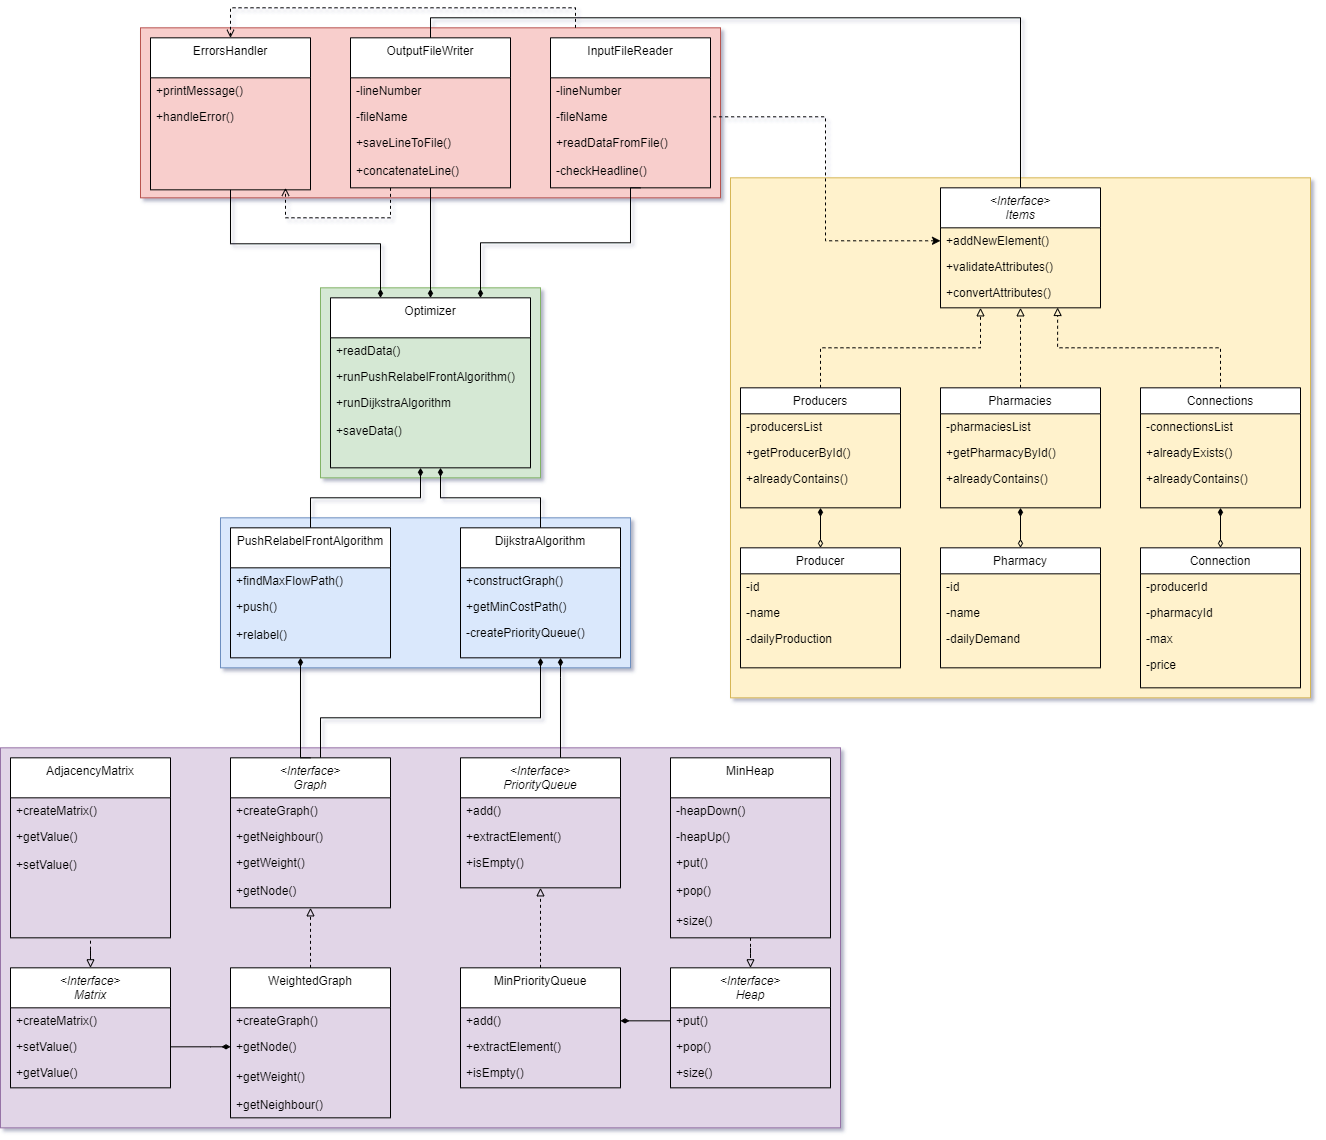
\includegraphics[width=15cm]{chart.png}
      \captionof{figure}{}
    \end{figure}


}

\section{Wykorzystane kolekcje}
{\fontsize{13}{13}\selectfont
      W programie zostaną zaimplementowane zarówno struktury danych, jak i abstrakcyjne typy danych:
    \begin{enumerate}
        \item Tablice
        
        W tablicach będą przechowywane elementy, których ani długość, ani kolejność nie będzie zmieniała się w trakcie działania programu. 
        \item Listy liniowe 
        
        Listy (interfejs List) będą wykorzystywane do przechowywania elementów, których długość nie jest znana lub często zmienia się w trakcie działania programu. W zależności od tego czy w dla danej kolekcji będzie potrzebny szybki dostęp do konkretnych elementów, czy szybka iteracja będzie wykorzystywana klasa ArrayList albo LinkedList.
        \item Graf
        
        Graf z wagami będzie reprezentował możliwości i sekwencje dostaw szczepionek. Wagami będą ceny szczepionek. Graf zostanie zaimplementowany za pomocą macierzy.
        \item Macierz
        
        Macierz będzie reprezentowana za pomocą tablicy dwuwymiarowej. Wartościami macierzy będą wagi ścieżek grafu (ceny szczepionek).
        
        \item Kolejka Priorytetowa
        
        Kolejka Priorytetowa (Priority Queue) stworzona zostanie w oparciu o kopiec binarny i będzie wykorzystana do zaimplementowania algorytmu Dijkstry. Będzie przechowywała wierzchołki grafu. Priorytetem kolejki będzie aktualnie wyliczona odległość od wierzchołka źródłowego.
        
        \item Kopiec binarny minimalny
        
        Kopiec będzie przechowywał elementy w taki sposób, że rodzic będzie mniejszy lub równy swojemu dziecku. Jest to spowodowane tym, że wyciągane elementy będą w kolejności od najmniejszego do największego, gdyż tego będzie wymagała kolejka.
    \end{enumerate}
    \lhead{Wykorzystane kolekcje}
}
\newpage

\section{Algorytmy}
\lhead{Algorytmy}
{\fontsize{13}{13}\selectfont
    \begin{enumerate}
        \item\textbf{Algorytm Dijkstry}
        
            Jest to algorytm do znajdowania najkrótszej ścieżki w grafie.
            
            \subsection{Algorytm Dijkstry - działanie}
            Algorytm ten polega na tym, aby dopóki nie zostanie opróżniona kolejka priorytetowa usuwać wierzchołek o \underline{najniższym} priorytecie (ten najbliżej wierzchołka źródłowego) oraz dla każdego sąsiada v wierzchołka u sprawdzał warunek:
            
            d[u] + w(u,v) < d[v]
            
            \setlength{\parindent}{0pt}
            Gdy ten jest prawdziny wykonywał instrukcję:
            
            d[v] = d[u] + w(u,v)
        
            
            Gdzie:
            \begin{itemize}
                \item tablica d przechowuje odległości od wierzchołka źródłowego do pozostałych.
                \item w(u,v) to waga krawędzi u,v.
            \end{itemize}

            \setlength{\parindent}{12pt}
            
            Na końcu tablica d będzie zawierała najkrótsze odległości między źródłem, a pozostałymi wierzchołkami.


            \subsection{Algorytm Dijkstry - złożoność}
            Złożoność czasowa algorytmu Dijkstry wynosi:
            
            \textbf{O(E * log V)}
            
            Gdzie:
            \begin{itemize}
                \item V - liczba wierzchołów,
                \item E - liczba krawędzi,
            \end{itemize}
            
            Złożoność ta jest mniejsza niż np. dla algorytmu Bellmana-Forda - O(|V| * |E|), gdyż algorytm Dijkstry nie działa poprawnie dla grafów o wagach krawędzi ujemnych (takie nie wystąpią w programie).


        \item\textbf{Algorytm Relabel-to-Front}
        
        Jest to jeden z najbardziej efektywnych algorytmów obliczania maksymalnego przepływu 
        \subsection{Algorytm Relabel-to-Front - działanie}
        
        W algorytmie wyróżnia się trzy podstawowe kroki:
        
        \begin{enumerate}
            \item Inicjacja
            \begin{itemize}
                \item Inicjowanie wysokości przepływu jako zero.
                \item Inicjowanie wysokości wierzchołka źródłowego równego sumie liczby wierzchołków w grafie.
                \item Inicjowanie przepływu każdej krawędzi jako zero.
            \end{itemize}
            \item Push
            
            Operacja push polega na przesłaniu całej możliwej ilości nadmiarowego przepływu z u do v w krokach:
            \begin{itemize}
                \item Odjęcie ilości przepływu, która zostanie przesłana dalej.
                \item Dodanie przepływu do wierzchołka do którego przesyłamy.
                \item Dodanie przepływu do krawędzi (u,v).
                \item Odjęcie przepływu od krawędzi przeciwnej, aby zachować skośną symetrię.
            \end{itemize}
            \item Relabel
            
            Operacja relabel polega na zwiększaniu wysokości wierzchołka na którym wykonywana jest operacja do momentu aż będzie o 1 większa od najniższego sąsiada.
            
        
            W wersji algorytmu relabel-to-front w pełni rozładowujemy wierzchołek przed przejściem do kolejnego.

        \end{enumerate}
        
        \subsection{Algorytm Relabel-to-Front - złożoność}
            Złożoność czasowa algorytmu Relabel-to-Front wynosi:
            
            \textbf{O($V^3$)}
            
            Gdzie:
            \begin{itemize}
                \item V - liczba wierzchołów,
            \end{itemize}
            
            Złożoność ta jest mniejsza zarówno dla swojej podstawowej wersji push-relabel - O($V^2$) i znacznie mniejsza od złożoności algorytmu Edmondsa-Karpa - O(V * $E^2$).
        
    \end{enumerate}

}


\section{Pozostałe informacje}
{\fontsize{13}{13}\selectfont
    \begin{itemize}
        \item Program będzie działał w konsoli.
        \item Program nie będzie prowadził z użytkownikiem dialogu.
        \item Program będzie wymagał tylko jednego argumentu w linii polecenia - nazwy pliku wejściowego.
        \item Program będzie kończył działanie po wykryciu błędu i wyświetleniu komunikatu.
        
    \end{itemize} 

}
\lhead{Pozostałe informacje}

\end{document}
